% ch14b Quantum phase transitions, part b (书页 306-316 / 分册p018-028)
% 术语约定（供装配一致性核对）：phase-only model=纯相位模型；quantum rotor model=量子转子模型；
% Bose metal=玻色金属；quantum disordered regime=量子无序区；quantum critical regime=量子临界区；
% IST=绝缘体–超导体转变；dangerously irrelevant operator=危险无关算符；BKT/Berezinskii–Kosterlitz–Thouless 保留英文。
%--TAIL--
到一个中间区域，在其中热涨落而非量子涨落决定动力学。在此区域中，逆关联长度随温度线性变化，且其系数是普适的。该区域被称为量子临界区，因为系统正试图判定两个基态中哪一个更可取。处于这种不定态的一切体系的一个基本特征是：所有能标——或等价地，所有弛豫速率——随温度线性标度。因此，正如引言中所讨论的，在量子临界区，准粒子激发并非良定义的。随着 $\Delta$ 增大，系统从量子临界区交叉过渡到量子无序区。在这一极限下，温度退居次要地位，序参量的量子涨落决定物理。于是 $\langle\psi^{*}(\mathbf{r})\psi(\mathbf{r})\rangle\propto\exp(-r/\xi)\propto\exp(-mr)$。此区域中的能量激发是有能隙的，由 $\epsilon_{k}=\sqrt{k^{2}+m^{2}}$ 给出。

\section{输运性质}

电导率既是频率的函数，也是温度的函数。到临界点的距离同样决定着电导率。于是有 $\sigma=\Sigma(\hbar\omega,T,\Delta)$。考虑 $\Delta=0$ 的简单情形。零温输运性质应当如何确定？由于量子临界点出现在 $T=0$，合理的假设似乎是：正确的 $T=0$ 极限由 $\Sigma(\hbar\omega,T=0,0)$ 得到，而直流电导率则通过取零频极限获得。这当然假定了频率依赖与温度依赖是解耦的。若二者确实解耦，则 $\omega\to0,\,T=0$ 与 $\omega=0,\,T\to0$ 这两个极限便可交换次序。

Damle 与 Sachdev 在一篇开创性的论文 [DS1997] 中证明，在量子临界点附近，这两个极限毕竟不可交换。他们的论证基于如下观察：在量子临界点附近，电导率是 $\hbar\omega/k_{\mathrm{B}}T$ 的普适函数。这意味着 $\Sigma(\hbar\omega/k_{\mathrm{B}}T)$ 存在两个截然不同的 $T\to0$ 极限：一个极限是 $\Sigma(\hbar\omega\to0,T=0)=\Sigma(\infty)$，另一个是 $\Sigma(\omega=0,T\to0)=\Sigma(0)$。Damle 与 Sachdev 的要点在于 $\Sigma$ 是单调函数，因而 $\Sigma(0)\neq\Sigma(\infty)$。实验上，直流输运性质的一切测量都是在 $\hbar\omega\ll k_{\mathrm{B}}T$ 的极限下进行的，因此与实验相关的是 $\Sigma(0)$ 这一极限。早期关于绝缘体–超导体转变的全部理论工作 [C1991; WZ1990; KZ1993; W1994] 都基于极限形式 $\Sigma(\infty)$。该极限对应于相干区域，即高频极限，其中由外加电场引起的弛豫决定输运性质。然而相反的区域在性质上截然不同。在极限形式 $\Sigma(0)$ 中，热激发准粒子之间的碰撞支配一切弛豫过程。为描述这一区域，必须针对准粒子散射建立一个量子动理学方程（quantum kinetic equation），它与为金属中声子主导的输运所建立的玻尔兹曼方法直接类似。这里的关键意外在于：若不分析有限温弛豫过程，便无法理解 $T=0$ 量子临界点的输运性质。

为说明频率与温度趋于零这两个极限的不可交换性会如何剧烈地影响电导率，考虑量子无序区。在此区域中 $m\gg T$，能隙之上存在热激发的准粒子。然而，按朴素的考虑，能隙的存在意味着直流电导率应当为零。但事实并非如此。量子无序区中 $m\gg T$ 的约束意味着相关动量满足 $k<\sqrt{mT}<m$。于是色散关系可以写成
\begin{equation*}
\epsilon_{\mathbf{k}}\approx m+\frac{k^{2}}{2m}\approx m,\quad m\gg T,\tag{14.54}
\end{equation*}
而准粒子统计在量子无序区成为玻尔兹曼型的。因此，准粒子的布居指数地小。然而，准粒子布居的这种指数式稀少同时也导致指数式小的散射概率。精确计算 [DP2001] 表明，在量子无序区，散射率
\begin{equation*}
\frac{1}{\tau}=\pi T\,\mathrm{e}^{-m/T}\tag{14.55}
\end{equation*}
与动量无关，并由同一个压制准粒子布居的指数因子支配。由爱因斯坦关系，电导率是准粒子密度与散射时间的乘积。两个指数因子相互抵消 [DP2001]，给出电导率
\begin{equation*}
\sigma_{\mathrm{qd}}=\frac{2}{\pi}\,\frac{4e^{2}}{h}\tag{14.56}
\end{equation*}
它在 $m\ll1$ 时有限。在离临界点更远处，该系数会被相互作用的具体形式修正。尽管如此，直流电导率仍然保持有限。此外，散射率中的所有对数贡献 [DP2001] 在低温下都消失，因而不影响 $T=0$ 处有限的直流电导率。这一论证的关键在于：一旦准粒子服从玻尔兹曼统计，散射事件便变得稀少。因此，准粒子可以在不发生散射的情况下游弋相当长的距离。于是，纯相位模型（phase-only model）的普遍相图（图 14.5）包含一个作为超导体的有序相，以及一个“金属的”相位无序区。这个“绝缘体”是一个具有有限直流电导率的金属。这是频率与温度趋于零极限的不可交换性所引出的关键意外之一。Green 与 Sondhi [GS2005] 也利用上面讨论的相消论证证明，有能隙的即量子无序的相实际上是金属性的。我们把这个相称为玻色金属（Bose metal），因为其基本激发是玻色子。在有限频率下，$\Sigma(\omega,T)$ 在 $\omega=0$ 处呈现一个洛伦兹型峰，其宽度为 $1/\tau$ 的量级。因此，实验观测玻色金属所受的约束是 $\omega\ll1/\tau$。温度为 0.1 K 时，弛豫时间为 $10^{10}\exp(-m/T)\ \mathrm{s}^{-1}$，其中 $m\gg T$。测量直流电导率时的典型实验频率为 2--27 Hz 的量级。因此，只要 $T>0.05m$，玻色金属便可以被观测到。典型情况下 $T>0.1m$。由此可见，似乎不存在任何关于频率的实验约束会妨碍对玻色金属相的观测。然而，这里描述的玻色金属是脆弱的，因为所有其他散射机制（例如无序）都会破坏导致式 (14.56) 的完美相消。因此，绝缘体–超导体转变尚待解决的问题之一，便是低温下居间金属相的起源。

\begin{figure}[H]\centering
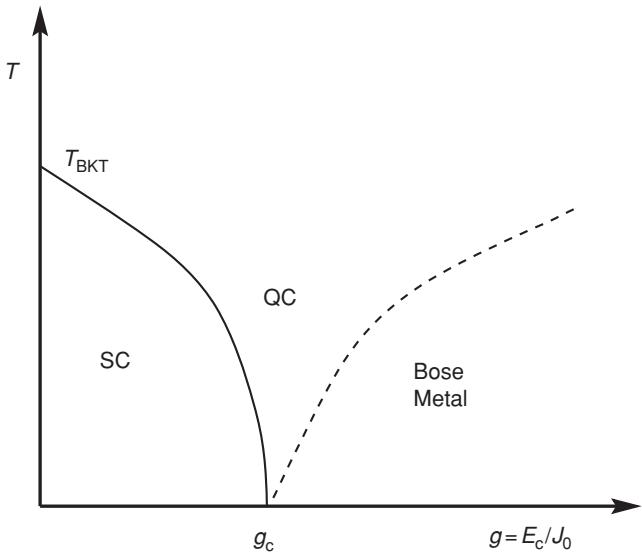
\includegraphics[width=0.6\textwidth]{figs/ch14/fig_14.5.jpg}
\caption*{图 14.5\quad 约瑟夫森结阵列中相位相干性被破坏的相图。对该体系，$g$ 由充电能量 $E_{\mathrm{C}}$ 与约瑟夫森耦合 $J_{0}$ 之比给出。$T_{\mathrm{BKT}}$ 是 Berezinskii–Kosterlitz–Thouless（BKT）温度，低于该温度时相位相干性得以建立；$g_{\mathrm{c}}$ 则给出为破坏超导相所需的相位无序的临界值。QC 指量子临界区，其中逆关联长度随温度线性变化。一旦相位相干性被破坏，便出现金属态。该金属态完全源于电导率的频率趋于零极限与温度趋于零极限之间缺乏可交换性。}\label{fig:auto:14.5}
\end{figure}

\section{实验}

纯相位模型对薄膜中绝缘体–超导体转变（insulator-superconductor transition，IST）的适用性，取决于在转变两侧都存在库珀对这一前提。因此，直接测量单粒子谱的隧穿实验是检验纯相位模型关键预言的理想手段。在颗粒薄膜上进行的这类实验 [B1994] 揭示：在转变的绝缘一侧，单粒子能隙保持有限，且相对体超导值并无衰减。因此，纯相位模型对颗粒薄膜中实验观测到的 IST 给出了准确的描述。

\begin{figure}[H]\centering
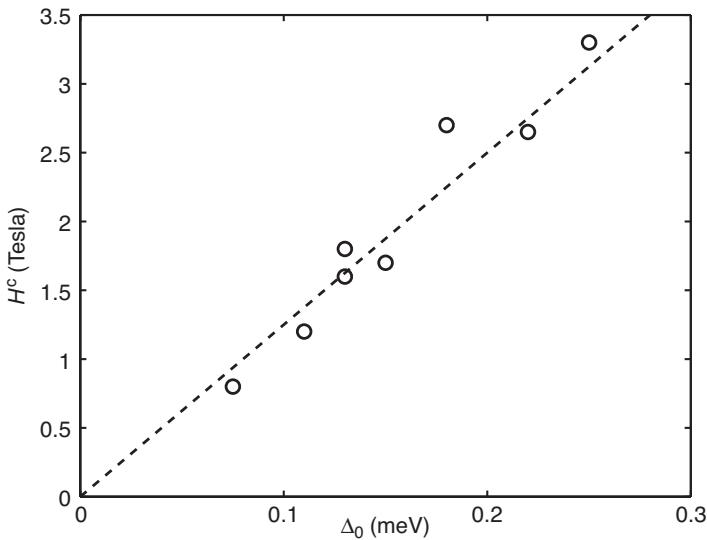
\includegraphics[width=0.55\textwidth]{figs/ch14/fig_14.6.jpg}
\caption*{图 14.6\quad PbBi/Ge 薄膜的临界磁场 $H_{\mathrm{c}}$ 对能隙 $\Delta_{0}$ 的关系图。根据 S.-Y. Hsu 的学位论文 [H1995] 重绘。}\label{fig:auto:14.6}
\end{figure}

那么，均匀无序的薄膜情形又如何呢？这里的情况颇为不同。图 14.6 给出了 PbBi/Ge 中破坏超导态所需的临界磁场随单粒子能隙的变化。显而易见，$H_{\mathrm{c}}$ 随能隙线性标度。只要 $H_{\mathrm{c}}$ 对应于库珀对破坏场 $H_{\mathrm{c2}}$，这一对应关系便在 BCS 理论的预期之内（见式 (12.207)）。事实上，Valles 及其合作者 [HCV1995] 已确定：在 $H_{\mathrm{c}}$ 处，费米能处的态密度为其正常态值的 80\%，这正是 $H_{\mathrm{c}}\approx H_{\mathrm{c2}}$ 时应有的情形。因此，样品中有相当大的一部分不含库珀对。这一观察也与 Dynes 及其合作者的一系列实验 [V1992] 相符：在这些实验中，能隙被观测到在名义临界场 $H_{\mathrm{c}}$ 处消失。对 MoGe，Yazdani 与 Kapitulnik [YK1995] 也发现 $H_{\mathrm{c}}\approx H_{\mathrm{c2}}$。总体而言，这些观察意味着：在均匀无序薄膜中，由库珀对破坏产生的类电子准粒子布居于转变的绝缘一侧。因此，要描述这些体系，必须有超越纯相位模型的物理。

这一状况其实也可以从如下实验事实推断出来：在大批均匀无序薄膜中，临界点处的电阻率 $R_{\mathrm{c}}$ 等于正常态电阻率 $R_{\mathrm{N}}$。图 14.7 给出了 Bi [GM1998] 与 MoGe [YK1995] 样品 $R_{\mathrm{c}}$ 对 $R_{\mathrm{N}}$ 的典型曲线图。正常态电阻 $R_{\mathrm{N}}$ 是 [YK1995; GM1998] 由 $T>T_{\mathrm{p}}$ 的输运测量提取的（见图 14.3）。因此，在这一温区内大量存在的只有类电子激发。临界电阻 $R_{\mathrm{c}}$ 则在远低于 $T_{\mathrm{p}}$ 的温度下提取，它表示 $R(T)$ 随调控参量的曲线族在 $T\to0$ 时单一交叉点处的电阻率。在 Bi 与 MoGe 两种薄膜中，磁场诱发 IST。从 Bi 与 MoGe 两者的数据显而易见，$R_{\mathrm{c}}\approx R_{\mathrm{N}}$。除非在 $R_{\mathrm{c}}$ 处发生了向正常基态的转变，否则这种 $R_{\mathrm{c}}\approx R_{\mathrm{N}}$ 的对应没有理由出现。由于 $R_{\mathrm{N}}$ 关联于不存在库珀对的高温物理，$R_{\mathrm{c}}\approx R_{\mathrm{N}}$ 这一事实意味着：在这些均匀无序薄膜中，绝缘态必定含有类电子准粒子。此外，在所有情形中 $R_{\mathrm{c}}$ 都略高于 $R_{\mathrm{N}}$，介于 $900\,\Omega$ 与 $8000\,\Omega$ 之间。这些数值与纯相位模型所预言的玻色子电阻量子 $h/4e^{2}=6500\,\Omega$ 显然相差悬殊，进一步表明起作用的是超越纯相位模型的物理。

\begin{figure}[H]\centering
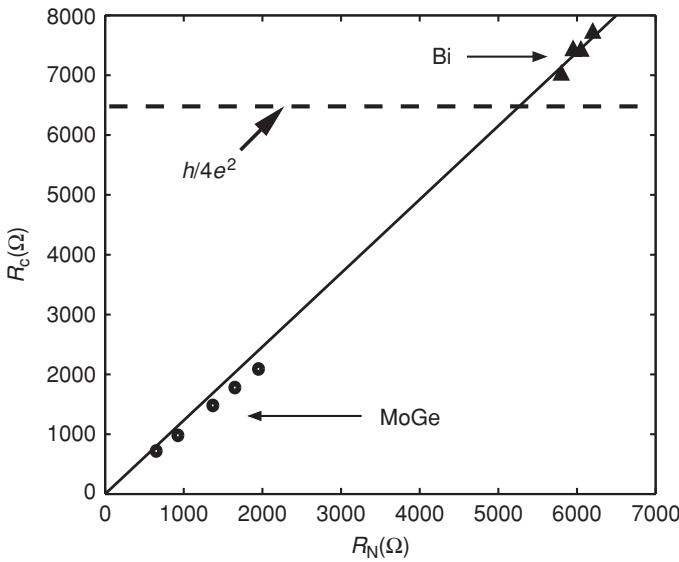
\includegraphics[width=0.55\textwidth]{figs/ch14/fig_14.7.jpg}
\caption*{图 14.7\quad Bi [GM1998] 与 MoGe [YK1995] 样品的临界电阻 $R_{\mathrm{c}}$ 随正常态电阻 $R_{\mathrm{N}}$ 的变化。转变处不存在普适值以及 $R_{\mathrm{c}}$ 与 $R_{\mathrm{N}}$ 之间的相关性表明：向绝缘态的转变中含有类电子准粒子，这正是高温正常态的特征。}\label{fig:auto:14.7}
\end{figure}

总而言之，纯相位物理似乎足以描述颗粒薄膜。然而，对大多数均匀无序薄膜，实验指向一个由类电子准粒子布居的绝缘态。因此，对破坏（pair-breaking）似乎是驱动 IST 的主导机制。由此，3d XY 模型便不再足以描述均匀无序薄膜中的 IST，因为绝缘体中存在无能隙的电子激发。在这种情形下，临界电阻便不必由 $2e$ 玻色子的电阻量子 $R_{\mathrm{Q}}=h/4e^{2}$ 界定，正如实验所观测的那样。把正常电子纳入 IST 的进展，可沿着 Feigelman 与 Larkin [FL1998] 新近采取的路线取得。

\section{标度与T线性电阻率}

量子相变受 $T=0$ 量子临界点支配。此外，由于温度起着关键作用，量子相变相应的场论是 $(d+z)$ 维的。量子转子模型是刻画超导体–非超导体量子临界点附近相互竞争的基态之间本质张力的最简单模型。该模型可以改写为金兹堡–朗道理论。$T=0$ 量子临界点的一个关键意外之处在于：输运性质必须由热激发准粒子之间的碰撞来决定。就量子转子模型而言，把准粒子散射纳入进来，会在量子无序区导致一个金属相。只要无序不是对破坏型的，玻色金属相对弱无序就是稳定的。

\begin{figure}[H]\centering
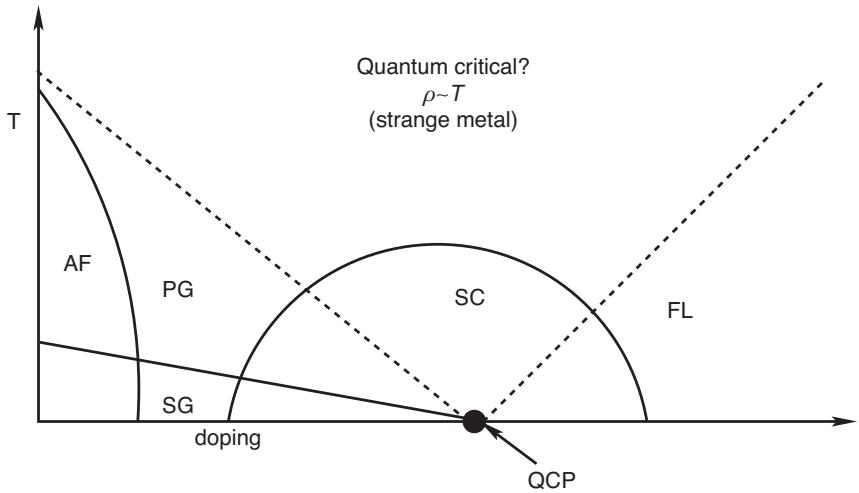
\includegraphics[width=0.72\textwidth]{figs/ch14/fig_14.8.jpg}
\caption*{图 14.8\quad 高温铜氧化物超导体的示意相图，以温度和空穴浓度（掺杂）为变量。各相为：AF 表示反铁磁体，SG 表示自旋玻璃，SC 表示具有 $d_{x^{2}-y^{2}}$ 对称性的超导体。自旋玻璃相终止于穹顶内部的一个临界掺杂水平（量子临界点，QCP）。虚线表示交叉过渡而非临界行为。在此图中，PG 与 FL 分别表示赝能隙相与费米液体相：前者的单粒子谱发展出一个凹陷，后者的输运性质变得更为常规。漏斗形区域中的奇异金属行为——$T$ 线性电阻率——曾被归因于量子临界行为。然而，对量子临界点处电导率的标度分析排除了这一情形。}\label{fig:auto:14.8}
\end{figure}

在量子临界点正上方，动力学由温度决定。因此，人们很自然地倾向于把随温度线性的电阻率与量子临界点可能的存在联系起来，铜氧化物超导体（cuprate）即属此列 [BTKW1993]。铜氧化物中的 $T$ 线性电阻率至今仍是正常态物理中的关键挑战。在铜氧化物理论的早期，人们曾引入基于某种量子临界性的解释 [T1999; V1989] 来说明 $T$ 线性电阻率。可以问一个简单的问题：量子临界性是否对由此得到的电阻率的形式施加任何限制？确实施加，这从下面的标度分析即可看出。

这一论证 [PC2005] 基于三条一般性假设：(1) 临界自由度携带电流；(2) 临界点附近只有一个长度标度是相关的；(3) 电荷守恒。倘若属实，这些假设便排除将量子临界性作为 $T$ 线性电阻率成因的可能。

考虑一个一般的作用量 $S$，只要电流是临界的，其微观细节并不重要。外加电磁矢势 $A^{\mu}$（$\mu=0,1,\ldots,d$）与电流 $j_{\mu}$ 耦合，使得
\begin{equation*}
S\to S+\int \mathrm{d}\tau\, d^{d}x\, A^{\mu}j_{\mu}.\tag{14.57}
\end{equation*}
这里的关键是矢势与电流线性耦合，因而其标度维数为 1。这一事实在后面的证明中至关重要。在量子体系的一参数标度假设下，在小于关联体积 $\xi^{d}$ 的体积内的空间关联、以及在短于 $\xi_{t}\propto\xi^{z}$ 的时间标度上的时间关联都很小，尺度为 $\xi^{d}\xi_{t}$ 的时空区域表现为独立的块体。利用这一假设，通过清点整个体系中关联体积的数目，我们写出配分函数对数之奇异部分的标度形式：
\begin{equation*}
\ln Z=\frac{L^{d}\beta}{\xi^{d}\xi_{t}}\,F\bigl(\delta\xi^{d_{\delta}},\{A_{\lambda}^{i}\xi^{d_{A}}\}\bigr).\tag{14.58}
\end{equation*}

在此表达式中，$L$ 是系统尺寸，$\delta$ 是到临界点的距离，$d_{\delta}$ 与 $d_{A}$ 分别是临界耦合与矢势的标度维数。变量 $A_{\lambda}^{i}=A^{i}(\omega=\lambda\xi_{t}^{-1})$ 对应于标度频率 $\lambda=\omega\xi_{t}$ 处的（均匀、$k=0$）电磁矢势，而 $i=1,\ldots,d$ 标记空间分量。把配分函数的对数对电磁规范场 $A^{i}(\omega)$ 取两次导数，
\begin{align*}
\sigma_{ij}(\omega,T)&=\frac{1}{L^{d}\beta}\ \frac{1}{\omega}\ \frac{\delta^{2}\ln Z}{\delta A^{i}(-\omega)\delta A^{j}(\omega)}\\
&=\xi^{-d}\ \frac{\xi_{t}^{-1}}{\omega}\ \xi^{2d_{A}}\ \frac{\delta^{2}}{\delta A_{-\bar{\lambda}}^{i}\delta A_{\bar{\lambda}}^{j}}\,F(\delta=0)\,\Big|_{\substack{\bar{\lambda}=\omega\xi_{t}\\ \{A_{\bar{\lambda}}^{i}=0\}}}\\
&=\frac{Q^{2}}{\hbar}\ \xi^{2d_{A}-d}\ \Sigma_{ij}(\omega\xi_{t}),\tag{14.59}
\end{align*}
便确定了电荷为 $Q$ 的载流子的电导率。我们已明确地取 $\delta=0$，因为我们关注的是量子临界区。在有限温度下，时间关联长度被温度截断为 $\xi_{t}\propto1/T$，且 $\xi_{t}\propto\xi^{z}$。如前所述，电磁规范场的工程量纲为 1（$d_{A}=1$）。这一结果完全源于电荷守恒 [W1992]。于是我们得到电导率的一般标度形式
\begin{equation*}
\sigma(\omega,T)=\frac{Q^{2}}{\hbar}\ T^{(d-2)/z}\ \Sigma\left(\frac{\hbar\omega}{k_{\mathrm{B}}T}\right)\tag{14.60}
\end{equation*}
其中 $\Sigma$ 只是比值 $\omega/T$ 的显函数。（为简单起见，$ij$ 张量指标已略去。）这一标度形式把 Wen [W1992] 导出的 $T=0$ 频率依赖的临界电导率推广到非零温度。这一般性标度形式，即式 (14.60)，也与 Damle 和 Sachdev [DS1997] 在其对量子临界点附近碰撞主导输运的详尽研究中所提出的形式一致（另见文献 [SS2000] 中的标度分析）。当前推导所清楚阐明的是：无论哈密顿量的底层统计或微观细节如何——无论它是玻色型的（如 Damle 与 Sachdev 的工作 [DS1997]）还是其他类型，无论有无无序——电导率的一般标度形式都保持不变。$d=2+\epsilon$ 维安德森金属–绝缘体转变（可视为以无量纲无序强度为调控参量的量子相变 [W1979; AALR1979]）的电导率（见式 (13.25)）服从这里导出的电导率标度函数。

在零频率即直流极限下，我们得到
\begin{equation*}
\sigma(\omega=0)=\frac{Q^{2}}{\hbar}\ \Sigma(0)\ \left(\frac{k_{\mathrm{B}}T}{\hbar c}\right)^{(d-2)/z}.\tag{14.61}
\end{equation*}
一般地 $\Sigma(0)\neq0$。否则，电导率将完全由自由能的非奇异、因而非临界的部分决定。铜氧化物是各向异性的三维体系。因此，对临界模式而言，相应的维数是 $d=3$ 而非 $d=2$。在后一种情形，温度前置因子是常数。对 $d=3$，我们发现仅当 $z=-1$ 时才得到 $T$ 线性电阻率。在标准的可交换（commutative）场论中，这样一个负的 $z$ 值是非物理的，因为它意味着在临界点处长波涨落的能标发散。

虽然假定 $\Sigma(0)$ 在零温下有限肯定合理，但 $\Sigma(0)$ 实际上发散也确有可能。出现这种情形的一个可能场景是：一个危险无关算符（dangerously irrelevant operator）支配着电导率。此时 $\Sigma(0)\sim1/T^{p}$，且当 $p=(d-2)/z+1$ 时得到 $T$ 线性行为。这只可能发生在上临界维数以上。在该区域，一切临界性都是平均场型的。因此，目前尚不能排除的一种可能性是：铜氧化物中的一切临界性本质上是平均场型的，而危险无关算符控制着电导率。然而，对强关联体系而言，临界性本质上是平均场型的可能性不大。

这一证明提示，下列三种可能性之一可能是相关的：(1) 量子临界性与该问题毫无关系；(2) 电流由非临界自由度携带；或 (3) 存在新的量子临界场景，其中额外的长度标度描写物理。在涉及非临界自由度的场景中，铜氧化物正常态的费米子载流子可以与一个临界玻色模式耦合。这样的解释类似于磁性体系中的情形 [H1976]：费米子从无质量玻色型密度涨落或自旋涨落上散射，导致电阻率的一系列代数形式 [K1996; R1999]，在反铁磁与铁磁体系中分别从 $T^{4/3}$ 变化到 $T^{3/2}$。虽然无序可以改变指数 [R1999]，但 $T$ 线性电阻率只在一个受限的参数空间中出现。铜氧化物中 $T$ 线性电阻率的稳健性使这类场景不太可能。我们所倡导的场景是额外长度标度进入问题的场景。这一额外自由度来自跨越莫特能隙的动力学谱权重转移。这将在最后一章中描述。

\section*{习题}
\addcontentsline{toc}{section}{习题}

\textbf{习题 14.1}\quad 在量子转子模型
\begin{equation*}
H=E_{\mathrm{C}}\sum_{i}\left(\hat{n}_{i}-n_{0}\right)^{2}-t\sum_{\langle ij\rangle}\left(b_{i}^{\dagger}b_{j}+b_{j}^{\dagger}b_{i}\right),\tag{14.62}
\end{equation*}
中，证明当 $n_{0}$ 不是整数时，相应的作用量具有如下形式：
\begin{equation*}
S\propto\int_{0}^{\beta}\mathrm{d}\tau\,\theta\partial_{\tau}\theta-\sum_{\langle ij\rangle}V(\cos\theta_{i}-\theta_{j}).\tag{14.63}
\end{equation*}
这一版本的量子转子模型称为无公度玻色–哈伯德模型（incommensurate Bose--Hubbard model）。这对动力学指数的取值有什么后果？

\textbf{习题 14.2}\quad 利用式 (14.35)，证明式 (14.36) 的结果。

\textbf{习题 14.3}\quad 利用 $C_{0}(\tau,\tau')$ 的低温形式，即式 (14.37)，建立式 (14.46) 中最后的等式。

\textbf{习题 14.4}\quad 完成式 (14.51) 中的积分，然后用泊松求和公式导出式 (14.52)。

\section*{参考文献}
\addcontentsline{toc}{section}{参考文献}

\begin{itemize}[leftmargin=2em,itemsep=0pt,parsep=0pt,label={}]
\item [AALR1979] E. Abrahams, P. W. Anderson, D. C. Licciardello, and T. V. Ramakrishnan, \emph{Phys. Rev. Lett.} \textbf{42}, 673 (1979).
\item [AR1998] G. Aeppli and T. F. Rosenbaum, in \emph{Dynamical Properties of Unconventional Magnetic Systems}, eds. A. T. Skjeltorp and D. Sherrington (Kluwer Academic Publishers, Netherlands, 1998), p. 107.
\item [A1964] P. W. Anderson, in \emph{Lectures on the Many Body Problem}, ed. E. R. Caianiello (Academic, New York, 1964), Vol. 2, p. 127.
\item [B1994] R. P. Barber, Jr., L. M. Merchant, A. La Porta, and R. C. Dynes, \emph{Phys. Rev. B} \textbf{49}, 3409 (1994).
\item [BTKW1993] For a review, see B. Batlogg, H. Takagi, H. L. Kao, and J. Kwo, \emph{Electronic Properties of High-$T_{c}$ Superconductors}, eds. H. Kuzmany, \emph{et al.} (Springer-Verlag, Berlin, 1993), p. 5.
\item [B1971] V. L. Berezinskii, \emph{Zh. Eksp. Teor. Fiz.} \textbf{61}, 1144 (1971) [\emph{Sov. Phys.-JETP} \textbf{34}, 610 (1971)].
\item [BMO1979] M. R. Beasley, J. E. Mooij, and T. P. Orlando, \emph{Phys. Rev. Lett.} \textbf{42}, 1165 (1979).
\item [C1991] M. C. Cha, M. P. A. Fisher, S. M. Girvin, M. Wallin, and A. P. Young, \emph{Phys. Rev. B} \textbf{44}, 6883 (1991).
\item [DP2001] D. Dalidovich and P. Phillips, \emph{Phys. Rev. B} \textbf{64}, 052507 (2001).
\item [DS1997] K. Damle and S. Sachdev, \emph{Phys. Rev. B} \textbf{56}, 8714 (1997).
\item [D1981] S. Doniach, \emph{Phys. Rev. B} \textbf{24}, 55063 (1981).
\item [FL1998] M. V. Feigelman and A. I. Larkin, \emph{Chem. Phys.} \textbf{235}, 107 (1998).
\item [F1972] R. P. Feynman, \emph{Statistical Mechanics} (W. A. Benjamin, Reading, Mass., 1972), p. 66.
\item [FH1965] R. P. Feynman and A. R. Hibbs, \emph{Quantum Mechanics and Path Integrals} (McGraw-Hill, New York, 1965), p. 42.
\item [F1990] M. P. A. Fisher, \emph{Phys. Rev. Lett.} \textbf{65}, 923 (1990).
\item [GM1998] For a review, see A. M. Goldman and N. Markovic, \emph{Physics Today} \textbf{51} (11) 39 (1998).
\item [GS2005] A. G. Green and S. L. Sondhi, \emph{Phys. Rev. Lett.} \textbf{95}, 267001 (2005).
\item [HN1979] B. I. Halperin and D. R. Nelson, \emph{J. Low Temp. Phys.} \textbf{36}, 5999 (1979).
\item [HP1990] A. F. Hebard and M. A. Paalanen, \emph{Phys. Rev. Lett.} \textbf{65}, 927 (1990).
\item [H1976] J. A. Hertz, \emph{Phys. Rev. B} \textbf{14}, 1165 (1976).
\item [H1995] S.-Y. Hsu, Ph.D. Thesis, Brown University, 1995.
\item [HCV1995] S.-Y. Hsu, J. A. Chervenak, and J. M. Valles, Jr., \emph{Phys. Rev. Lett.} \textbf{75}, 132 (1995).
\item [H1959] J. Hubbard, \emph{Phys. Rev. Lett.} \textbf{3}, 77 (1959).
\item [J1989] H. M. Jaeger, D. B. Haviland, B. G. Orr, and A. M. Goldman, \emph{Phys. Rev. B} \textbf{40}, 182 (1989).
\item [K1996] S. Kambe, S. Raimand, L.-P. Regnault, \emph{et al.}, \emph{J. Phys. Soc. Jpn.} \textbf{65}, 3294 (1996).
\item [KZ1993] A. P. Kampf and G. T. Zimanyi, \emph{Phys. B} \textbf{47}, 279 (1993).
\item [KT1973] J. M. Kosterlitz and D. J. Thouless, \emph{J. Phys. C} \textbf{6}, 1181 (1973).
\item [P1979] P. Pfeuty, \emph{Phys. Lett. A} \textbf{72}, 245 (1979).
\item [PC2005] P. Phillips and C. Chamon, \emph{Phys. Rev. Lett.} \textbf{95}, 107002 (2005).
\item [R1999] A. Rosch, \emph{Phys. Rev. Lett.} \textbf{82}, 4280 (1999).
\item [S1999] S. Sachdev, \emph{Quantum Phase Transitions} (Cambridge University Press, Cambridge, 1999).
\item [SS2000] T. Schneider and J. M. Singer, \emph{Phase Transition Approach to High Temperature Superconductivity: Universal Properties of Cuprate Superconductors} (Imperial College Press, London, 2000), p. 238.
\item [S1980] E. Simanek, \emph{Phys. Rev. Lett.} \textbf{45}, 1442 (1980).
\item [S1958] R. L. Stratanovich, \emph{Sov. Phys. Dokl.} \textbf{2}, 416 (1958).
\item [T1999] J. T. Tallon, J. W. Loram, G. V. M. Williams, \emph{et al.}, \emph{Phys. Stat. Sol. (b)} \textbf{215}, 531 (1999).
\item [V1992] J. M. Valles, Jr., R. C. Dynes, and J. P. Garno, \emph{Phys. Rev. Lett.} \textbf{69}, 3567 (1992).
\item [V1989] C. M. Varma, P. B. Littlewood, S. Schmitt-Rink, and A. E. Ruckenstein, \emph{Phys. Rev. Lett.} \textbf{63}, 1996 (1989).
\item [W1994] M. Wallin, E. S. Sorensen, S. M. Girvin, and A. P. Young, \emph{Phys. Rev. B} \textbf{49}, 12115 (1994).
\item [W1979] F. J. Wegner, \emph{Z. Phys. B} \textbf{35}, 207 (1979).
\item [W1992] X.-G. Wen, \emph{Phys. Rev. B} \textbf{46}, 2655 (1992).
\item [WZ1990] X. G. Wen and A. Zee, \emph{Intl. J. Mod. Phys. B} \textbf{4}, 437 (1990).
\item [W1965] B. Widom, \emph{J. Chem. Phys.} \textbf{43}, 3892 (1965).
\item [YK1995] A. Yazdani and A. Kapitulnik, \emph{Phys. Rev. Lett.} \textbf{74}, 3037 (1995).
\end{itemize}
